%!TEX root=../main.tex
\chapter{Climbing Mont Blanc Improvements}
\label{ch:improvements}

In this chapter it is assumed that a web interface follows the \gls{mvc} pattern. As briefly mentioned in sub-section \ref{subsec:cmb-arch-frontend}, Angular structures the HTML and Javascript code according to the \gls{mvc} pattern, and the reader should have the abstraction in mind when reading about browser or frontend implementations.

\section{Real Time Updates}
\label{sec:real-time}
The frontend view changes when a user performes actions against the frontend models as mentioned in sub-section \ref{subsec:cmb-arch-frontend}. However, the frontend view presented to a given user does not update automatically as other users interract and changes their data models, as models is stored locally in each of the user's browser. If the updated model contains data that should be known\footnote{Hereby known as \textit{shared data}.} to all users, the users does not get notified about the model changes dynamically and views may therefore display out of date information. Figure \ref{fig:update-problem} shows an example of the problem, as Alice updates some of her browser's model data when she interacts with the system. If Alice changes some data present in Bob's models, Bob will not be notified of the changes as all data transfer are done with HTTP requests between Alice and the server. However, Bob can fetch up to date data by manually refreshing his webpage. \\

\begin{sidewaysfigure}
    \centering
    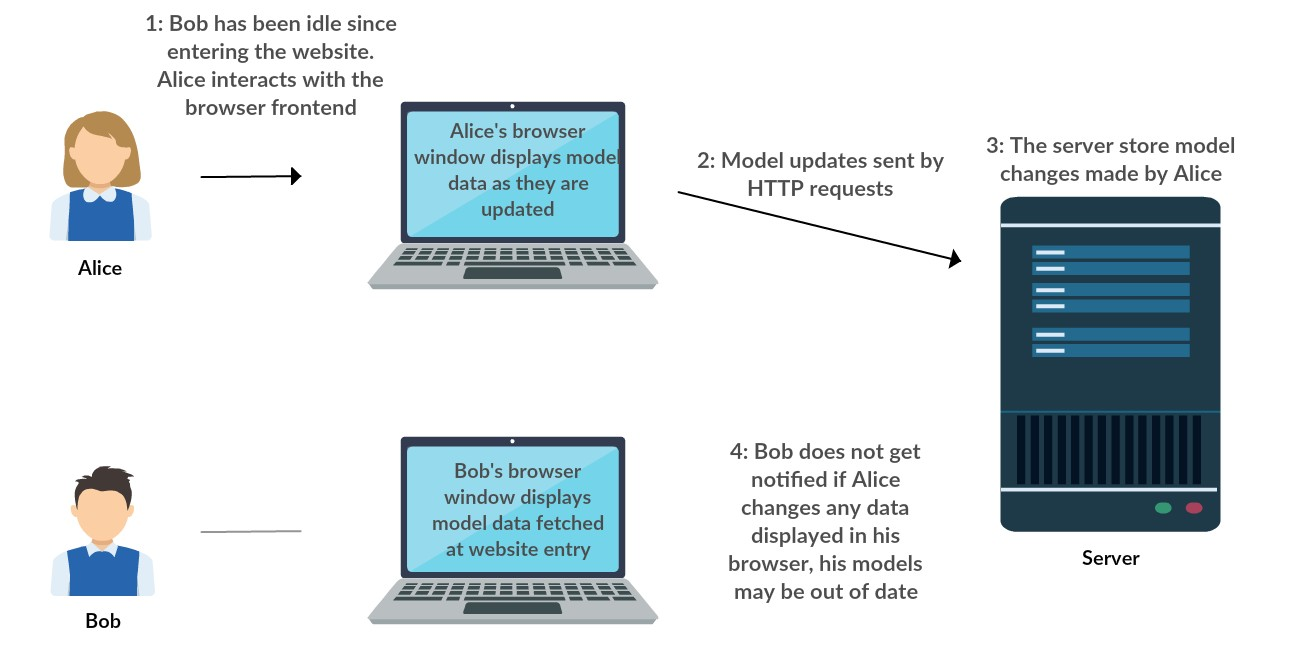
\includegraphics[width=1\textwidth]{figs/update_problem.jpg}
    \caption{Example of updating models without model change notifications}
    \label{fig:update-problem}
\end{sidewaysfigure}

Many websites requires to share data between multiple clients and dynamically notify clients if there are changes to the data. As an example in the \gls{cmb} system, it would be nice if the frontend interface dynamically updated as a user's submission finished running at the backend. In the old system before the improvements, the user had to manually refresh by clicking at a refresh button provided by the user interface or manually refresh the webpage. However, this section presents a technology which has been introduced in the new version of the system in order to dynamically update data relevant for multiple clients. \\

Socket.io \cite{SOCKETIO} is an \gls{api} for enabling real time communication between the server and connected clients. The \gls{api} was first made as Javascript library, but many open source projects have developed modules for other programming languages integrating the Socket.io \gls{api}. One benefit of the \gls{api} is that it works as a wrapper around a set of real time communication protocols to enable support for different browsers, which means that the framework can automatically detect the protocol supported by a client and use that information to select the best fitted communication protocol. \\

Rohit Rai states the communication protocols supported by the Socket.io \gls{api} \cite{Rai2013}. Figure \ref{fig:cmb-protocols} shows the communication protocols enabled in the new version of \gls{cmb}. The WebSocket protocol \cite{a:Fette2011}, shown in Figure \ref{fig:websocket}, has become more popular since its introduction in 2011 and is now supported by the most popular browsers. The protocol is a bit different from the well known HTTP protocol, as there is a persistent connection, or socket, between the client and the server as long as both entities are connected to the socket. The socket connection is closed if the client closes the browser window or the server goes down, or if the code explicitly indicates to close the socket. WebSockets enables easy two-way communication by letting two entities emit (read: send) messages back and forth on the socket connection, and respond differently depending on the type of message emitted on the socket. \\

Polling and long-polling both use the HTTP protocol and may seem similar at first glance. However, in long-polling, the server keeps the connection between the two entities open until there is an update to the requested data as shown in Figure \ref{fig:long-polling}. In polling, as shown in Figure \ref{fig:polling}, the client continuously requests data with some constant delay between each request, while the server respond on each request with the data currently stored at the server. Independent of the protocol, we can think of the connection between the server and client(s) and think of it as a "socket". \\

\begin{figure}
    \centering
    \begin{subfigure}[b]{1.0\textwidth}
        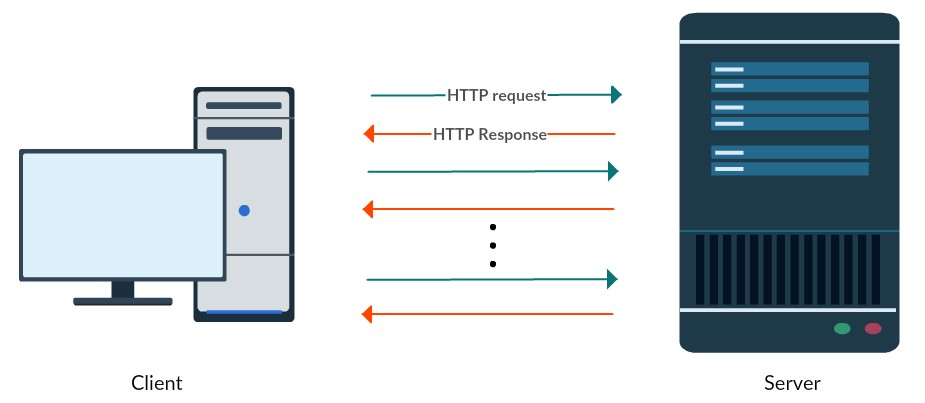
\includegraphics[width=\textwidth]{figs/polling.jpg}
        \caption{Polling: The client sends a series of HTTP request and the server responds on each request.}
        \label{fig:polling}
    \end{subfigure}
    ~ %add desired spacing between images, e. g. ~, \quad, \qquad, \hfill etc.
    %(or a blank line to force the subfigure onto a new line)
    \begin{subfigure}[b]{1.0\textwidth}
        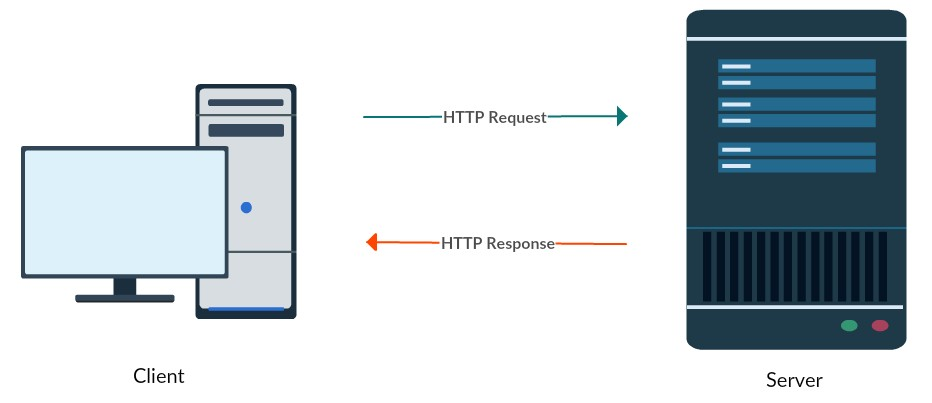
\includegraphics[width=\textwidth]{figs/long_polling.jpg}
        \caption{Long-polling: The client sends an HTTP request to fetch new data, the server holds the connection open until the requested data is updated.}
        \label{fig:long-polling}
    \end{subfigure}
    \begin{subfigure}[b]{1.0\textwidth}
        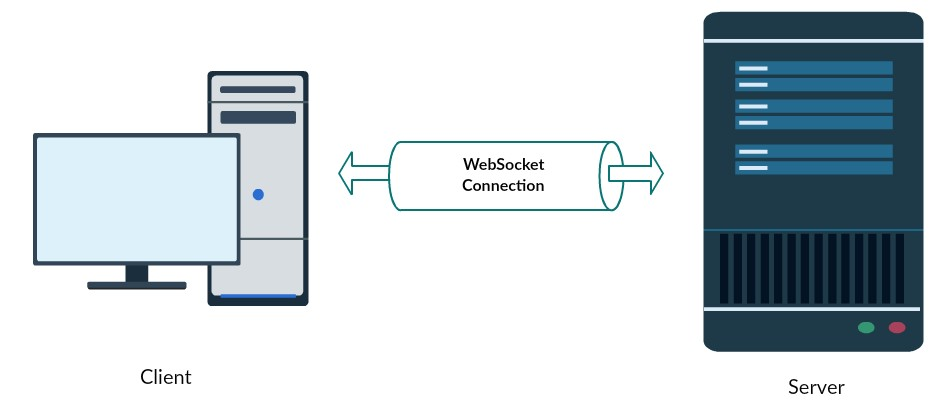
\includegraphics[width=\textwidth]{figs/websocket.jpg}
        \caption{WebSocket protocol: a two-way connection tunnel open throughout the whole client session. TCP is used as a transport protocol.}
        \label{fig:websocket}
    \end{subfigure}
    \caption{\gls{cmb} Socket.io communication protocols}\label{fig:cmb-protocols}
\end{figure}

Each socket can be "\textit{namespaced}" into separate communication channels within an application. A namespace can be viewed as a endpoint or network path, for example in the new \gls{cmb} prototype the namespace \textit{/cmb} is used as default namespace to emit messages between the client and the server. Every client initiating a socket on the namespace receives all messages emitted to the namespace, which makes it easy to share information between the server and clients connected to the namespace. \\

Each namespace can also define a set of \textit{rooms}, which can be viewed as sub-channels of a given namespace. A client needs to explicitly join a room to receive the messages emitted in a given sub-channel. Figure \ref{fig:namespaces-and-rooms} illustrates the concept. Each message emitted to the namespace \textit{/cmb} are received by both client one and two. Client three will only receive those messages emitted to the namespace \textit{/test}. If a message are emitted to room one within the \textit{/cmb} namespace, only client one will receive the message. \\

Socket.io also lets the programmer define \textit{events}, which can be emitted between the server and connected clients. Table \ref{tab:cmb-socketio-events} shows the events currently defined for the \gls{cmb}, and the actions taken either by the server or client depending on which enitity that emitted the event. The actions are only taken if the code defines event listeners for each event, and for the frontend it depends on the view that is displayed in each users' browser. As an example, the submission events shown in Table \ref{tab:cmb-socketio-events} are only valid if a given user is viewing the problem-screen shown in Figure \ref{}. This makes sense, because we are trying to do real time updates to the highscore list and the user's own submissions while he or she stays in the problem-screen. Events will therefore not be received if the users navigates to another view, as Socket.io event listeners in the frontend code are bound to views or rather the views' controllers.  \\

The two sub-sections below describes the technologies used by the server and frontend in order to support real time communication with Socket.io.

\begin{table}[t!]
    \centering
    \begin{tabular}{ | c | c | c | p{3.5cm} | }
    \hline
    \textbf{Event Name} & \textbf{Emitted by} & \textbf{Received by} & \textbf{Action}\\
    \hline
    \textit{join-problem} & Client(s) & Server & Server adds the client to the problem room specified in the emitted message. \\ \hline
    \textit{leave-problem} & Client(s) & Server & Server removes the client from the problem room specified in the emitted message. \\ \hline
    \textit{submission-deleted} & Server & Client(s) & Client fetches updated submission data from the server. \\ \hline
    \textit{submission-enqueued} & Server & Client(s) & Client displays a message in the browser window, notifying about queue size and information present in the emitted message. \\ \hline
    \textit{submission-dequeued} & Server & Client(s) & Client displays a message in the browser window, notifying about queue size and information present in the emitted message. \\ \hline
    \textit{submission-finished} & Server & Client(s) & Client loads own submissions as well as possible updates to the highscore list. \\ \hline
    \end{tabular}
    \caption[\gls{cmb} Socket.io events and corresponding actions]{\gls{cmb} Socket.io events and corresponding actions. Each submission event is sent within a room which simply is the database id of a given problem. Since we have one room per problem, we know that all submission events within a room has information about submissions made to a given problem.}
    \label{tab:cmb-socketio-events}
\end{table}

\begin{figure}
    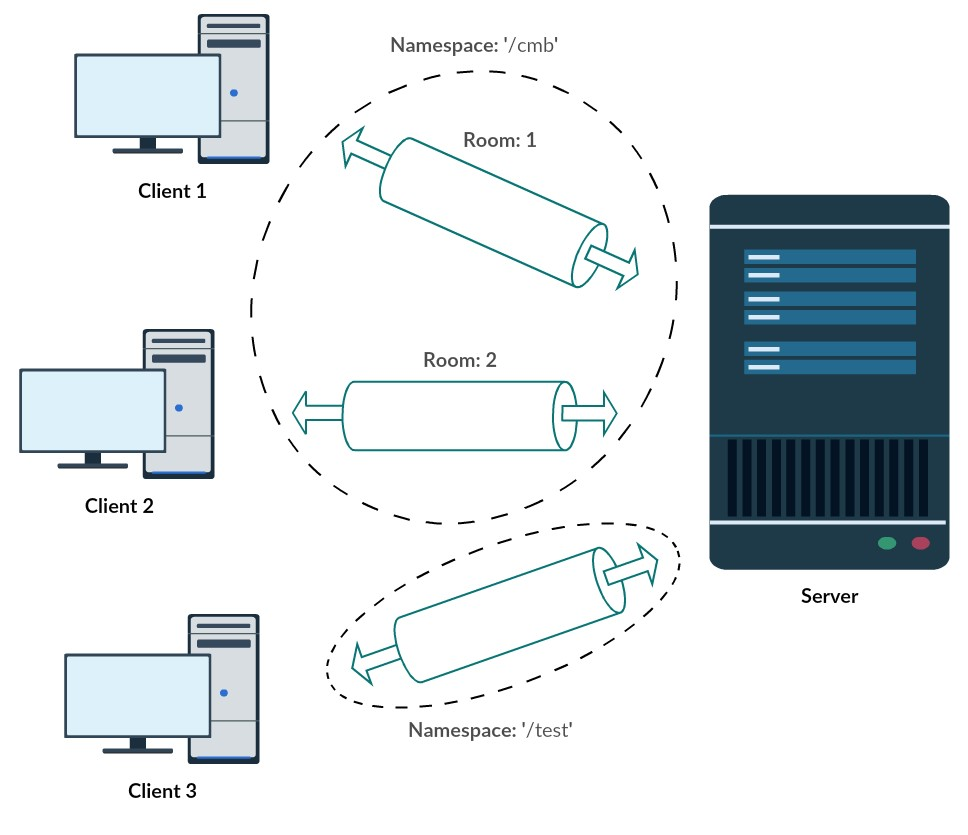
\includegraphics[width=1.0\textwidth]{figs/namespaces_and_rooms.jpg}
    \caption[Socketio namespaces and rooms in the \gls{cmb} system]{Socketio namespaces and rooms in the \gls{cmb} system. }
    \label{fig:namespaces-and-rooms}
\end{figure}

\subsection{Frontend Technology}
The frontend uses the client Socket.io library \cite{SOCKETIO} through a existing Angular component called \texttt{angular-socket-io} provided by Brian Ford \cite{ANGULARSOCKETIO}. The component is used to define a Angular \textit{factory}, which is simply a component that gathers and structures the setup of Socket.io in the client into a single service. The defined factory can then be used by other components in the Angular app, by marking components as dependent of the Socket.io factory. \\

\subsection{Server Technology}
The Python module Flask-SocketIO \cite{FLASKSOCKETIO} enables Flask applications to use the SocketIO \gls{api}. In addition, the modules gevent \cite{GEVENT} and gevent-websocket \cite{GEVENTWEBSOCKET} is installed in combination with the Socket.io module to enable the use of the WebSocket protocol. Gevent is a coroutine based networking library providing a high-level synchronous API on top of a asynchronous webserver. Asynchronous coroutines is used to handle multiple concurrent requests from multiple clients, and is required by the Flask-SocketIO module to support the WebSocket transport. \\

To fully support the WebSocket protocol Gunicorn also needs to make use a custom gevent worker supporting the WebSocket protocol. As stated by Miguel Grinberg on the Flask-Socketio documentation website, Gunicorn can only enable one worker due to limitations in the implemented load balancing algorithm. The Gunicorn load balancing algorithm cannot simply handle multiple workers and persistent WebSockets connections, which limits us to one worker per server. However, the worker uses coroutines to handle multiple concurrent requests as stated above. The gevent worker is enabled on the development server of \gls{cmb}, which also required some changes to the Nginx setup to fully support the WebSocket protocol. Appendix \ref{apdx:setup} describes setup information necessary to setup servers with Gunicorn and Nginx, while section \ref{sec:eval-tech} discusses pros and cons with selected technologies as well as presenting alternatives to the selected technology stack.

\section{Frontend}
\label{sec:impr-frontend}
This section will present figures of the views in the frontend that have changed in the new version of the system. The below sub-sections will explain the improvements and updates done to the views. The views not mentioned here has not been

\subsection{Bug Fixes}
Upload fixes in frontend
Sorting bug

\subsection{Views and Feedback}
Spinners + better error messages. Symbols added for usability. Bulletin board to display administrator messages. Colored feedback messages.

Figure \ref{} shows active bulletins

\subsection{Group Functionality Improvements}
JSON stat file download. Gathered group functionality.

\section{Server}
\label{sec:impr-server}
\subsection{Database Management System Updates}
The old version of \gls{cmb} used SQLite \cite{SQLITE} as \gls{dbms} at both the development and production server. SQLite is a lightweight \gls{dbms} which requires minimal configuration before use and is therefore popular to use during automatic unit testing, which also is done in the \gls{cmb} system. The initial goal were to improve, and thereby possibly change, the \gls{dbms} into a more sophisticated system. However, during the Spring the \gls{cmb} team found it uneccassery to change the \gls{dbms} of performance reasons and we found it more important to extend the system with new features. \\

Unrelated to the performance reasons, a new \gls{dbms} was wanted by the \gls{cmb} team and the IDI Department. We therefore changed the \gls{dbms} to MySQL due to its usage in other applications developed at the IDI Department. IDI provided the databases used by the system, and we also gained access to a database adminstrator interface available at \url{https://phpmyadmin.idi.ntnu.no/}. SQLAlchemy made the switch onto the new \gls{dbms} easy as it has a predefined MySQL adapter, and had no problems in setting up the new databases for our development and production servers. Further, Flask-Migrate \cite{FLASKMIGRATE}, used for database \textit{migrations}\footnote{Database magration is the task of managing versions of a database schema without altering previously stored database content.}, also worked without any changes in configuration. \\

A complete database dump were made from the SQLite databases. All SQL \texttt{INSERT} statements in the database dump were extracted and executed against the new development and production databases, to move all previously stored data in the SQLite databases over to the MySQL databases. The actions were performed with a combination of terminal commands and the database admin interface provided by IDI. MySQL and SQLAlchemy has not had any performance issues in the IDI Department, so the system uses the standard MySQL adapter provided by SQLALchemy. Implementing and enabling non-blocking database access has been added back to the backlog found in Appendix \ref{apdx:backlog} as a performance improvement.

\subsection{Database Schema Updates}
\label{subsec:impr-database}
The updates to the previous database schema is shown in Figure \ref{fig:updated-database-schema}. The Submissions-table have been updated with two new fields. The ``detailed state''-field was added to provide more information about a run to the user. In the current improved system, it contains a detailed string about a submissions state as it returns from the backend as explained in section \ref{sec:impr-backend}. The field can be modified in the future to store \gls{json} instead of simple text, if more information about a submission becomes available when executing code on the backend. \textit{Future developers should stribe to always keep users up-to-date with the state of their submissions}, and the new field aims to enable such feedback as explained in the section \ref{sec:impr-frontend} above. \\

\begin{figure}
    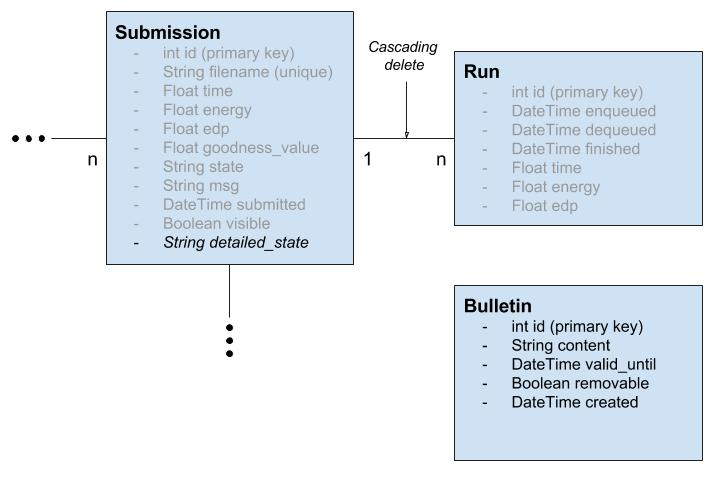
\includegraphics[width=0.9\textwidth]{figs/updated_database_schema.jpg}
    \caption[Database schema updates]{Database schema updates. The figure does only include the tables that are updated. Added table columns are highlighted. }
    \label{fig:updated-database-schema}
\end{figure}

A Bulletin-table were added to enable administrators to notify users about news and system messages. Bulletins has a field called \textit{valid\_until} which indicates until which date a given bulletin is valid, and the field is used to select the valid bulletins as explained in the below sub-section and is also displayed in the frontend as explained in section \ref{sec:impr-frontend} above. \\

Cascading deletes has also been added between the Submission- and Run-tables. This ensures that all rows in the Run-table associated with a Submission-row gets deleted upon delition of a submission, which ensures that there are no dangling rows in the Run-table and the database is left in a consistent state after deleting submissions. This is particularly important as both administrators and users are able to delete submissions.

\subsection{Routes}
The routes that has been updated or added to the \gls{rest}ful \gls{api} is listed in Table \ref{tab:cmb-updated-routes}. Figure \ref{fig:postman-request} shows an example GET-request against one of the routes defined in the table, which fetches data from a local server. The table does not include changes made to \gls{api} routes due to the implementation of the real time update improvement explained in section \ref{sec:real-time}, as the improvements does not change the internal logic of the original routes and has only added code to emit events. \\

\begin{figure}[h!]
    \centering
    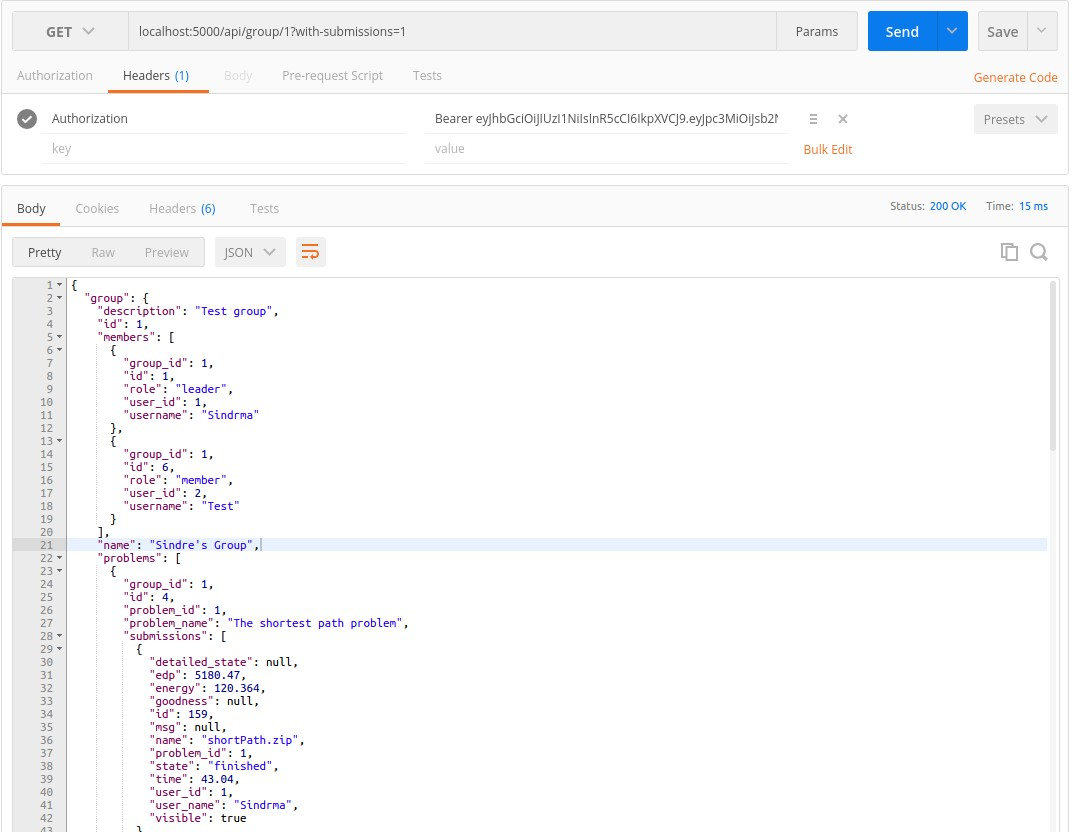
\includegraphics[width=1.0\textwidth]{figs/postman_request.jpg}
    \caption[Example request against local API]{Example request against local \gls{api} using Postman \cite{POSTMAN}. The request executes the GET-request \url{http://localhost:5000/api/group/1?with-submissions=1} presented in Table \ref{tab:cmb-updated-routes} with the query parameter \texttt{with-submissions} equal to one to also include the submissions made by the members of the group.}
    \label{fig:postman-request}
\end{figure}

\begin{table}[h!]
    \centering
    \begin{tabular}{ | c | c | p{4cm} | }
    \hline
    \textbf{\gls{api} Route} & \textbf{Method} & \textbf{Description} \\
    \hline
    \textit{/api/submission/$<$int:sub\_id$>$} & DELETE & If the submission with the given \texttt{id} exists and have been created by the current logged in user, the submission is deleted from the database as well as the file system. Requires login.\\ \hline
    \textit{/api/group/$<$int:group\_id$>$} & GET & Fetches information about a group by \texttt{id} depending on login status. If the user is not logged in, only public group information can be fetched. However, if the user is logged in, the user can also request information about private groups. If the query parameter \texttt{with-submissions} is set equal to 1, submissions made from group members is included in the response if the user is either a group member or leader. The response for leaders also include those submissions set to be unvisible. \\ \hline
    \textit{/api/bulletins} & GET & Returns all created bulletins. \\ \hline
    \textit{/api/bulletins/active} & GET & Returns all bulletins currently active. \\ \hline
    \end{tabular}
    \caption[\gls{cmb} API route updates with responses]{\gls{cmb} API route updates with responses. The routes listed shows the substring necessary to query the \gls{api}, and need to be combined with the \textit{path} of the server providing the \gls{api}. For example to delete a submission with \texttt{id} 1 from the development server \gls{api}, a delete request needs to be made against \url{http://climb-dev.idi.ntnu.no/api/submission/1}.}
    \label{tab:cmb-updated-routes}
\end{table}
\clearpage
\subsection{Admin Interface}
Several new problems have been added to the system during the Spring semester. Most problems were added due to a master thesis of two students, assessing the \gls{cmb} system's suitability for conducting digital exams in the course TDT4102 Procedural and Object-Oriented Programming \cite{TDT4102}. However, during the Spring we had a lot of trouble making the newly added problems solvable, as some submissions locked the backend infinetely. It turned out that some of the administrators had uploaded input and answer files with CR/LF (DOS) line endings, which locked the checker program during parsing of the input and answer files. The checker locked itself as the backend and server is Unix based systems and uses Unix line endings (LF). \\

The bug is removed in the new admin interface. When uploading files to the server, the files are automatically converted into Unix files with LF line endings. This is done by running all input and answer files through the \texttt{vim} \cite{VIM} command \texttt{vim + "argdo set ff=unix | update" +wqa ./*.txt} in the directory containing the problem files. The checker source file is not run through the command as the g++ compiler handles both Unix and DOS filetypes. \\

In addition some errors occured when administrators tried to remove locked submissions in the database through the admin interface. Due to lack of training, it often left the database and the server file system in a inconsistent state. As explained above, cascading delete were added between the \texttt{Run} and \texttt{Submission} tables to partially solve the problem, but the files associated with a submission would still remain in the server file system and had to be removed manually. However, deletion of submission files were often forgotten and it caused filename conflicts if the user re-submitted zip files with equal folder and file names as a previous submission.\footnote{A suggested future improvement is presented in section \ref{sec:future-work}, which is based upon storing submission files by the uniquely generated database id instead of using user defined folder and file names.}\\

The Flask-Admin \cite{FLASKADMIN} procedure \texttt{on\_model\_delete} solves the above inconsistency problem. It has been added to handle when submissions are deleted from the database, and takes care of removing all files in the server file system assoociated with a deleted submission. However, it is still possible to leave the database in a inconsistent state if one do not use the admin interface to delete database content. If other tools than the Flask-Admin module are to be used in the future to handle database, SQLALchemy provides event listeners which can be used instead of the above mentioned procedure. As the \gls{cmb} team currently uses the admin interface to handle database content, the \texttt{on\_model\_delete} procedure in the Flask-Admin interface is used. \\

Administration of the Bulletin-table peresented in sub-section \ref{subsec:impr-database} has also been added using the Flask-Admin module. This is shown in Figure \ref{fig:admin-bulletin}, which shows how to create bulletins and how to view the bulletins stored in the database.

\begin{figure}
    \centering
    \begin{subfigure}[b]{0.48\textwidth}
        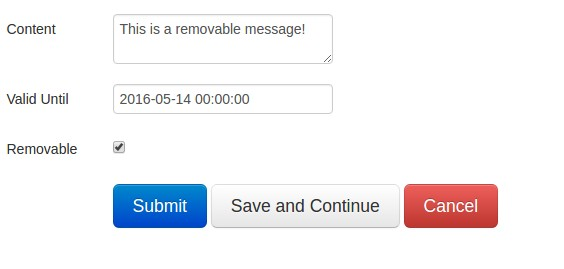
\includegraphics[width=\textwidth]{figs/bulletin_creation.jpg}
    \end{subfigure}
    ~ %add desired spacing between images, e. g. ~, \quad, \qquad, \hfill etc.
    %(or a blank line to force the subfigure onto a new line)
    \begin{subfigure}[b]{0.48\textwidth}
        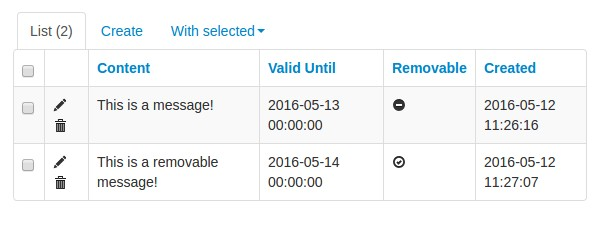
\includegraphics[width=\textwidth]{figs/bulletin_list.jpg}
    \end{subfigure}
    \caption{Bulletin creation and overview in the admin interface}
    \label{fig:admin-bulletin}
\end{figure}

\section{Backend}
\label{sec:impr-backend}
There have been some small changes in the backend code. The \gls{cmb} team discovered that there were no timeout when running the small correctness test, which could potentially lock the backend if the submitted code contained infinite loops. Locking the backend should not be acceptable under any condition, and the Unix program \texttt{timeout} \cite{TIMEOUT} is therefore used as during the big correctness test to kill the submitted program after some time if it stalls to long. Since the small input set is much smaller than the big correctness test, it is currently set to a third of the timeout of the big correctness or 30 seconds. \\

The \gls{json} returned by the backend is also slightly changed. A ``state'' field were added to better track the state of the program as it executes on the backend, especially if there is an error during execution. The field is currently used as input to the ``detailed state'' database field as described above, which is further used in the frontend to specialize the feedback given to the user if there is an error during execution of the program. Currently, the field is a simple string describing the state of the submitted program when the backend are done executing. A quick further discussion of the field and its potential are described in section \ref{sec:eval-tech}.

\section{Improvement Proposals}

\subsection{Stability Test}

\subsection{How-To Page and About Page}

\subsection{Adding Problems}

\subsection{Discussion Forum}
